To demonstrate this feature, we consider
decompression bombs, files that expand exponentially when decoded, consuming enormous
computation time in addition to their large memory footprint.
PNG files are vulnerable to such an attack, and although \textit{libpng} now
supports some mitigations~\cite{www-libpng-bombs}, one cannot always expect (or
trust) such functionality from third-party code.

We benchmarked the use of \textit{libpng}'s ``simple API'' to decode an in-memory PNG
file.  We then compared against synchronous isolation using preemptible functions, as
well as the na\"ive alternative mitigations proposed in Section~\ref{sec:intro}.  For
preemptible functions, we wrapped all uses of \textit{libpng} in a call to
\texttt{launch()} and used a dedicated (but blocking) reaper thread to remove the
cost of cancellation from the critical path; for threads, we used
\texttt{pthread\_create()} followed by \texttt{pthread\_timedjoin\_np()} and,
conditionally, \texttt{pthread\_cancel()} and \texttt{pthread\_join()}; and for
processes, we used \texttt{fork()} followed by \texttt{sigtimedwait()}, a
conditional \texttt{kill()}, then a \texttt{waitpid()} to reap the child.  We ran
\texttt{pthread\_cancel()} both with and without asynchronous cancelability enabled,
but the former always deadlocked.  The timeout was 10 ms in all cases.

\begin{figure}
	\begin{minipage}{0.235\textwidth}
	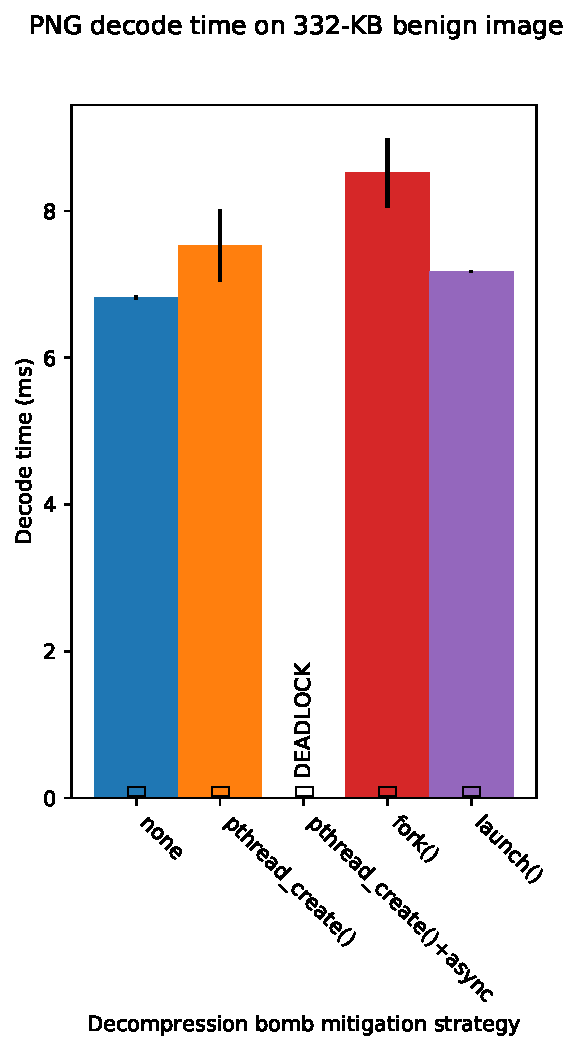
\includegraphics[width=\textwidth]{figs/cerberus2_nns16_surplus256k_mirjam}
	\subcaption{Benign image}
	\label{fig:libpng:benign}
	\end{minipage}
%
	\begin{minipage}{0.235\textwidth}
	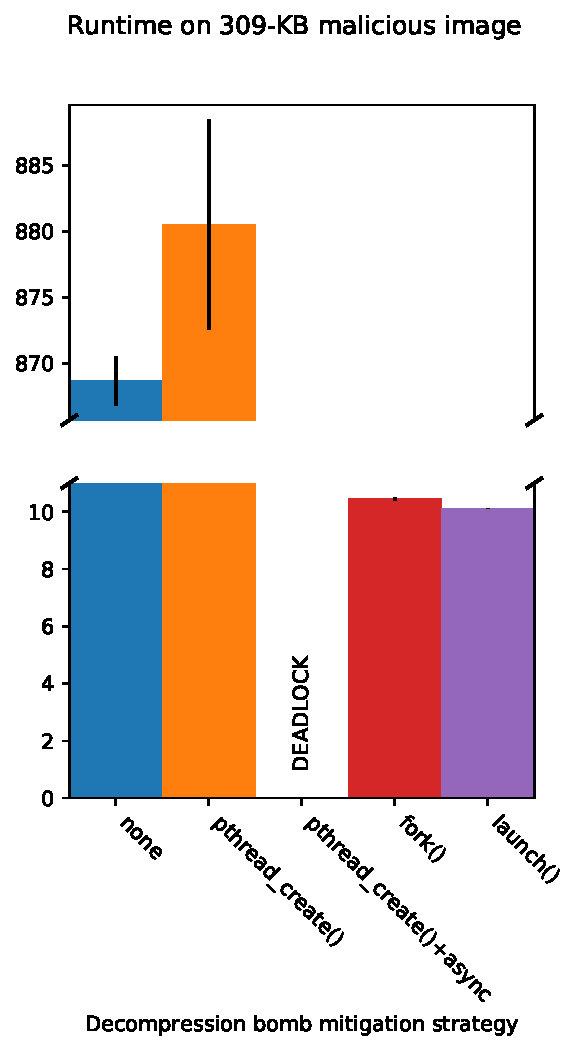
\includegraphics[width=\textwidth]{figs/cerberus2_nns16_surplus256k_10K}
	\subcaption{Malicious image}
	\label{fig:libpng:bomb}
	\end{minipage}
\caption{\textit{libpng} in-memory image decode times}
\end{figure}

Running on the benign RGB image \texttt{mirjam\_meijer\_mirjam\_mei.png} from version
\texttt{1:0.18+dfsg-15} of Debian's \texttt{openclipart-png} package showed
\texttt{launch()} to be both faster and lower-variance than the other approaches,
adding 355 $\mu$s or 5.2\% over the baseline (Figure~\ref{fig:libpng:benign}).  The
results for \texttt{fork()} represent a best-case scenario for that technique, as we
did not implement a shared memory mechanism for sharing the buffer, and the cost of
the system call will increase with the number pages mapped by the process (which was
small in this case).

Next, we tried a similarly-sized RGB decompression bomb from revision
\texttt{b726584} of \url{https://bomb.codes} (Figure~\ref{fig:libpng:bomb}).  Without
asynchronous cancelability, the pthreads approach was unable to interrupt the thread.
Here, \texttt{launch()} exceeded the deadline by just 100
$\mu$s, a figure that includes deviation due to the 100-$\mu$s preemption interval in
addition to \textit{libinger}'s own overhead.  It again had the lowest variance.

Applying preemptible functions to this problem proved easy:\@ the
\texttt{launch()}/\texttt{cancel()} approach took just 20 lines of Rust, including
the implementation of a reaper thread to move libset reinitialization off the
critical path.  In comparison, the \texttt{fork()}/\texttt{sigtimedwait()} approach
required 25 lines of Rust.  Note that due to their use of the
\textit{libpng} C library and use of zero-copy buffers, both benchmarks include
blocks of unsafe Rust.
